\begin{theorem}[Ramsey's Theorem]\label{thm:ramsey_two_colors}
	Let $\ell_1, \ell_2 \geq 2$, then there exists a non-zero $n \in \mathbb{N}$ such that $n \to (\ell_1, \ell_2)$.
\end{theorem}
\begin{proof}
	Clearly $\ell_1 \to (\ell_1, 2)$ and $\ell_2 \to (2, \ell_2)$ (after all either $K_{\ell_{i}}$ is monochromatic or there exist a monochromatic clique of order $2$). We will proceed using induction on $\ell_1 + \ell_{2}$, we may assume that $\ell_1 + \ell_2 \geq 6$, with $\ell_1, \ell_2 \geq 3$.
	Additionally by our induction hypothesis we may assume the existence of non-zero $n_1, n_2 \in \mathbb{N}$ such that $n_1 \to (\ell_1, \ell_2 - 1)$ and $n_2 \to (\ell_1 - 1, \ell_2)$. Next let $n := n_1 + n_2$ we will show that $n \to (\ell_1, \ell_2)$. Fix an arbitrary $2$-edge coloring $\chi$ on $K_n$ and let $v$ be a vertex in $K_n$, then $v$ is adjcent to $n - 1$ other vertices in $K_{n}$, hence:
	\begin{equation*}
		n_1 + n_2 - 1 = n - 1 = \abs{N_{\chi}(v; 1)} + \abs{N_{\chi}(v; 2)}
	\end{equation*}
	meaning either $\abs{N_{\chi}(v; 1)} \geq n_2$ or $\abs{N_{\chi}(v; 2)} \geq n_1$. Without loss of generality assume that the second inequality holds, namely $\abs{N_{\chi}(v; 2)} \geq n_1$. By our inductive hypothesis, the complete graph $G = (N_{\chi}(v; 2), N_{\chi}(v; 2) \times N_{\chi}(v; 2))$ contains either a $1$-monochromatic clique of order $\ell_{1}$ (in which case we are done) or a $2$-monochromatic clique of order $\ell_{2} - 1$, in which case we note that $v$ is connected to the vertices in $N_{\chi}(v; 2)$ via edges that $\chi$ assigns the color $2$, hence complete graph on the vertex set $N_{\chi}(v; 2) \cup \left\{v\right\}$ forms a $2$-monochromatic clique of order $\ell_{2}$.
\end{proof}

\begin{corollary}\label{cor:ramsey_for_arbitarily_many_colors}
	Let $\ell_1, \ell_2, \ldots, \ell_r \geq 2$, then there exists a non-zero $n \in \mathbb{N}$ such that $n \to (\ell_1, \ell_2, \ldots, \ell_{r})$.
\end{corollary}

\begin{proof}
	We proceed using induction on $r$, the base case $r = 2$ is proven in Theorem \ref{thm:ramsey_two_colors}.
	Next assume that the theorem holds for $r - 1$. From Theorem \ref{thm:ramsey_two_colors}, it follows that there exists a $\ell \in \mathbb{N}_{> 0}$ such that $\ell \to (\ell_{r - 1}, \ell_{r})$.
	By our induction hypothesis we may find a $n \in \mathbb{N}_{> 0}$ for which it holds that:
	\begin{equation*}
		n \to (\ell_1, \ell_2, \ldots, \ell_{r - 2}, \ell)
	\end{equation*}
	Now given any $r$-edge coloring $\chi$ on $K_n$ we may obtain a $r - 1$-edge coloring $\chi'$ on $K_n$ by defining:
	\begin{equation*}
		\chi'(e) = \begin{cases} \chi(e) & \text{ if } \chi(e) < r - 1 \\ r - 1 & \text{ otherwise } \end{cases}
	\end{equation*}
	Hence $\chi'$ must either emit a $i$-monochromatic clique of order $\ell_i$, for some $i \in \left\{1, 2, \ldots, r - 2\right\}$ (in which case we are done) or a $(r - 1)$-monochromatic clique of order $\ell$. Let $K_\ell$ be this monochromatic clique, then $\chi$ associates every edge in $G$ with either $r - 1$ or $r$. However $\ell$ was chosen so that $\ell \to (\ell_{r - 1}, \ell_r)$, hence $G$ must contain either a $(r - 1)$-monochromatic clique of order $\ell_{r - 1}$ or a $r$-monochromatic clique of order $\ell_{r}$.
\end{proof}

\begin{definition}
	The \textit{Ramsey number} $R(k_1, k_2, \ldots, k_{r})$, is the minimal $n \in \mathbb{N} \setminus \left\{0\right\}$ such that $n \to (k_1, k_2, \ldots, k_{r})$, additionally we let $R(k; r)$ denote $R(k_1, k_2, \ldots, k_{r})$, with $k_1 = k_2 = \cdots = k_r = k$.
\end{definition}
Generally direct computation of Ramsey numbers are extremely difficult,




\begin{example}\label{exmp:R3_3}
	In this example we will show that $R(3, 3) = 6$, we start by showing that $R(3, 3) \leq 6$. Consider the edge coloring $\chi: E(K_{6}) \to \left\{red, blue\right\}$ on $K_6$ and let $v$ be a vertex in $K_6$, then $v$ has $5$ adjacent neighbours, by the generalized pigeonhole principle, Theorem \ref{thm:gpp}, there is a color $c$ (either $red$ or $blue$) such that $\abs{N_{\chi}(v; c)} \geq 3$.

	Without loss of generality we may assume that $c = red$. Next take pairwise distinct $v_1, v_2, v_3 \in N_{\chi}(v; red)$, then we must have $\chi(v_{i}, v_{j}) = blue$ for pairwise distinct $i, j \in [3]$, since we otherwise would have that $K_{6} |_{\left\{v, v_i, v_j\right\}}$ would form a $red$-monochromatic clique of order $3$. However this in turn means that $\chi(v_i, v_j) = blue$ for all pairwise distinct $i, j \in [3]$, hence $K_6 |_{\left\{v_1, v_2, v_3\right\}}$ forms a $blue$-monochromatic clique of order $3$.

    On the other hand it is easy to construct a $2$-edge coloring on $K_5$ which emits no monochromatic subclique of order $3$, see for instance the graph in Figure \ref{fig:K5_counter_example}.
    \begin{figure}[H]
  \centering
  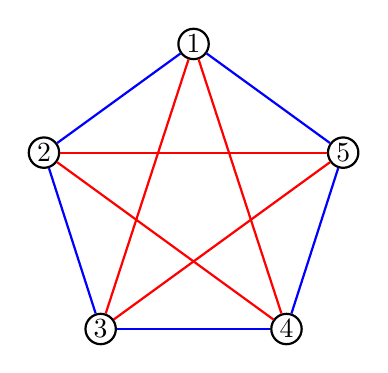
\begin{tikzpicture}
    \tikzset{punkt/.style={circle, thick, draw=black, minimum width=0.2cm,inner sep=1}}
    \node[punkt] at (0.0, 2.0) (a) {$1$};
    \node[punkt] at (-1.9, 0.62) (b) {$2$};
    \node[punkt] at (-1.18, -1.62) (c) {$3$};
    \node[punkt] at (1.18, -1.62) (d) {$4$};
    \node[punkt] at (1.9, 0.62) (e) {$5$};
    %\draw (0,0) circle [radius=2];

    % Blue edges
    \draw [thick, draw=blue] (a) -- (b);
    \draw [thick, draw=blue] (b) -- (c);
    \draw [thick, draw=blue] (c) -- (d);
    \draw [thick, draw=blue] (d) -- (e);
    \draw [thick, draw=blue] (e) -- (a);

    % Red edges
    \draw [thick, draw=red] (a) -- (c);
    \draw [thick, draw=red] (a) -- (d);
    \draw [thick, draw=red] (b) -- (d);
    \draw [thick, draw=red] (b) -- (e);
    \draw [thick, draw=red] (c) -- (e);
  \end{tikzpicture}
  \caption{A 2-edge coloring on $K_{5}$ that emits no monochromatic subclique of order $3$.}
  \label{fig:K5_counter_example}
\end{figure}
Finally since $R(3, 3) > 5$ and $R(3, 3) \leq 6$, we obtain that $R(3, 3) = 6$.
\end{example}
